\section{Introduction}
\subsection{What is return-oriented programming?} \label{sect:what}
\frame{
    \frametitle{Buffer overflow vulnerabilities}
    simple example:
    \begin{itemize}
        \item fixed size character buffer
        \item program reads a string from the keyboard and copies it to the buffer without bounds checking
        \item number of input characters $>$ buffer size \lto\ \bo
        \item variables on the stack are overwritten -- possibly including the current function's return address
        \item best case scenario: \pgm{SIGSEGV}
    \end{itemize}
}

\frame{
    \frametitle{Return-oriented programming}
    \begin{itemize}
        \item generalization of return-to-libc exploitation
        \item attacker uses \bo-vulnerability or something similar to inject return addresses into the stack
        \item \rtl-exploits chain together calls to library functions (\libc\ in most cases)
        \item \ro\ exploits jump a few instructions before a function's \ret\ to perform small operations
    \end{itemize}
    By carefully chaining together such jumps, an attacker can perform arbitrary computations!
}

\frame{
    \frametitle{Why care?}
    \begin{itemize}
        \item $45\%$ of all recorded security vulnerabilities in Ubuntu: \\
              \lto\ \bo\ vulnerabilities
        \item \bo\ exploits have been implemented in numerous malicious programs across different platforms
        \item Return-oriented programming:
              \begin{itemize}
                  \item probably the most advanced \bo\ exploitation technique so far
                  \item developed and refined over decades
              \end{itemize}
    \end{itemize}
}



\subsection{Before we begin...} \label{sect:terms}
\frame{
    \frametitle{Terms of service}
    \begin{itemize}
        \item Although I don't intend to, unfortunately I tend to
              \begin{itemize}
                  \item become overzealous,
                  \item talk too fast and
                  \item speak with a slur.
              \end{itemize}
              \lto\ Please insult me, if I do!
        \item By sitting here and listening to the talk, you agree that
              \begin{itemize}
                  \item you will not use the knowledge provided here to harm anyone,
                  \item I am not responsible for anything you break while messing around with the techniques I present,
                  \item \texttt{vim} is the name of the one true editor,
                  \item proprietary software is inherently evil.
              \end{itemize}
        \item Feel free to ask questions at any time.
    \end{itemize}
}

\frame{
    \frametitle{Stack diagrams}
    Stack diagrams are depicted from the stack's top to bottom:
    \begin{center}
        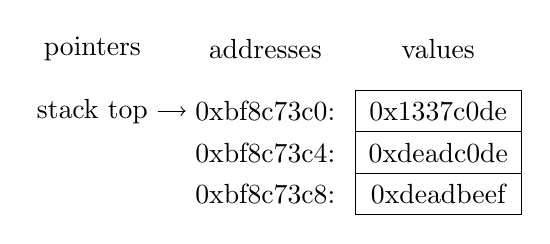
\begin{tikzpicture}
            \tikzset{x=2.5em, y=1.5em}
            \tikzstyle{mem}=[rectangle, draw, minimum width=6em, minimum height=1.5em]

            \draw (0.0, 3.5)    node        (l0)    {pointers};
            \draw (2.5, 3.5)    node        (l1)    {addresses};
            \draw (5.0, 3.5)    node        (l2)    {values};

            \draw (0.0, 2.0)    node        (esp0)  {stack top};
            \draw (2.5, 2.0)    node        (a2)    {0xbf8c73c0:};
            \draw (2.5, 1.0)    node        (a1)    {0xbf8c73c4:};
            \draw (2.5, 0.0)    node        (a0)    {0xbf8c73c8:};
            \draw (5.0, 2.0)    node[mem]   (s2)    {0x1337c0de};
            \draw (5.0, 1.0)    node[mem]   (s1)    {0xdeadc0de};
            \draw (5.0, 0.0)    node[mem]   (s0)    {0xdeadbeef};

            \draw [->]      (esp0) -- (a2);
        \end{tikzpicture}
    \end{center}
}

\frame{
    \frametitle{Platform}
    Examples and demo compiled and tested with
    \begin{itemize}
        \item \texttt{gcc} version 4.7.2
        \item \texttt{gdb} version 7.4.1
        \item \unit{32}{bit} Debian GNU/Linux 7.1 \\
              \lto\ instruction set architecture: IA-32
        \item Intel Core 2 Duo P7450
    \end{itemize}
}



\subsection{Examples} \label{sect:examples}
\frame{
    \frametitle{Computer worms}
    \begin{itemize}
        \item The \morris\ aka. "Great Worm"
              \begin{itemize}
                  \item utilized a \bo-vulnerability in the \pgm{fingerd} program on Unix systems
                  \item rendered infected systems unusable within 90 minutes
              \end{itemize}
        \item The \name{Slammer} worm
              \begin{itemize}
                  \item used \bo-vulnerabilities in Microsoft's "SQL Server 2000" and "Desktop Engine 2000"
                  \item infected roughly 75000 servers in approximately 30 minutes
                  \item caused network overloads on a great scale
              \end{itemize}
        \item The \name{Sasser} worm
              \begin{itemize}
                  \item exploited a vulnerability in Microsoft's LSASS
                  \item caused systems to shut down
              \end{itemize}
    \end{itemize}
}



\subsection{History} \label{sect:history}
\frame{
    \frametitle{Timeline of \bo\ exploits}
    \begin{itemize}
        \item[1988] \morris
        \item[1996] Aleph One: "Smashing The Stack For Fun And Profit"
        \item[1997] Solar Designer: \rtl\ basics
        \item[1998] Solar Designer: security patch for the Linux kernel
        \item[2000] PaX: Implementation of \wx
        \item[2001] Nergal: function chaining with \rtl
        \item[2007] Hovav Shacham: "Return-into-libc without function calls" \\
                    \lto\ \rop
        \item[since] more and more proof, that \rop\ is a real threat
    \end{itemize}
}
